% !TEX encoding = UTF-8
% !TEX TS-program = pdflatex
% !TEX root = ../tesi.tex

%**************************************************************
\chapter{Descrizione dell'applicativo}
\label{cap:applicazione}
%**************************************************************

In questo capitolo viene descritto l'applicativo le cui funzionalità sono state estese durante lo stage.\\

\section{Architettura serverless}
L'architettura della web app è basata sul \emph{Serverless Framework}, un \gls{framework} che permette di costruire architetture \gls{serverless}. Esso consente inoltre di definire l'architettura \gls{AWS} attraverso un file in formato \gls{YAML}. \\
 Nei paragrafi seguenti vengono mostrati alcuni esempi della sintassi per la definizione delle infrastrutture necessarie ai nuovi servizi implementati ed il procedimento da seguire per effettuare il \gls{deploy} della struttura \gls{serverless}.
	\subsection{Definizione delle resources}
	Attraverso la direttiva \emph{ Resources} è possibile definire le risorse a cui le funzioni \emph{Lambda} possono accedere, ovvero tabelle \emph{DynamoDB} e \emph{bucket S3} .
	
		\subsubsection{Tabelle DynamoDB}
		\begin{figure}[H]
			\centering
			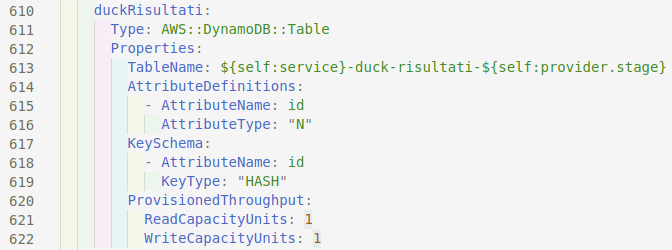
\includegraphics[width=11cm]{immagini/tabellaDB.png} \\
			\caption{\label{fig:tabellaDB} Esempio del codice per la creazione di una tabella DynamoDB}
		\end{figure}
		
		Nel codice sopra riportato:
		\begin{itemize}
			\item \textbf{Type} definisce il tipo di risorsa da creare;
			\item \textbf{TableName} indica il nome della tabella riportato nei servizi \gls{AWS};
			\item \textbf{AttributeDefinitions} descrive gli attributi che compongono la chiave primaria;
			\item \textbf{KeySchema} definisce la struttura della chiave primaria. Nell'esempio la chiave è composta da un solo attributo ma DynamoDB permette di definire anche chiavi più complesse;
			\item \textbf{ProvisionedThroughput} specifica il numero di letture e scritture permesse della risorsa.
		\end{itemize}

		\subsubsection{Bucket S3}
			
		\begin{figure}[H]
			\centering
			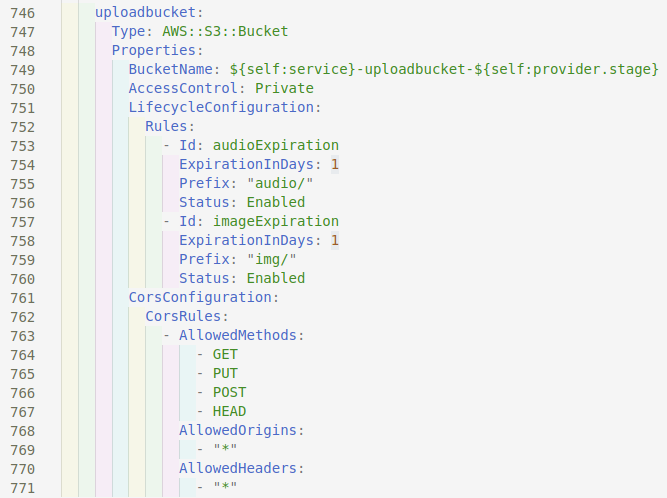
\includegraphics[width=11cm]{immagini/bucketS3.png} \\
			\caption{\label{fig:bucketS3} Esempio del codice per la creazione di un bucket S3}
		\end{figure}
	
		Nel codice sopra riportato:
		\begin{itemize}
			\item \textbf{Type} definisce il tipo di risorsa da creare;
			\item \textbf{BucketName} indica il nome del \emph{bucket} riportato nei servizi \gls{AWS};
			\item \textbf{AccessControl} specifica i permessi di accesso al \emph{bucket};
			\item \textbf{LifeCycleConfiguration} permette di definire delle regole per il ciclo di vita degli oggetti all'interno del bucket. Nel caso riportato sono state definite due regole per due diversi prefissi all'interno del \emph{bucket} (\emph{audioExpiration} e \emph{imageExpiration}) entrambe con durata di un giorno;
			\item \textbf{CorsConfiguration} descrive le configurazione per le \gls{CORS} per gli oggetti del \emph{bucket}.
		\end{itemize}
	
	\subsection{Definizione delle funzioni Lambda}
	Per definire le funzioni \emph{Lambda} viene utilizzata la direttiva \emph{functions}. 
	
	\begin{figure}[H]
		\centering
		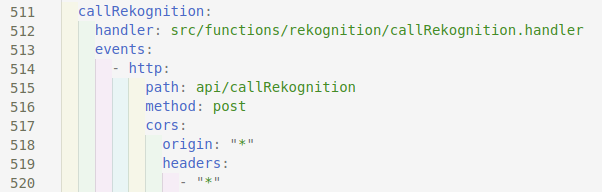
\includegraphics[width=11cm]{immagini/lambda.png} \\
		\caption{\label{fig:lambda} Esempio del codice per la creazione di una funzione Lambda}
	\end{figure}

	Nel codice sopra riportato:
	\begin{itemize}
		\item \textbf{handler} è il riferimento al file contenente il codice della funzione; 
		\item \textbf{events} indica gli eventi che causano l'esecuzione della funzione \emph{Lambda}. Specificando \item \textbf{Http} permette di definire degli \emph{API Gateway} HTTP endpoint che quando chiamati provocano l'esecuzione della funzione;
		\item \textbf{path} definisce il path dell'endpoint e identifica la risorsa;
		\item \textbf{method} indica il tipo di accesso HTTP permesso;
		\item \textbf{cors} abilita le \gls{CORS}.
	\end{itemize}
	
	\subsection{Deploy del back-end}
	Per effettuare il \gls{deploy} delle modifiche alle funzioni e alle risorse definite nel file \emph{serverless.yml} è sufficiente eseguire il comando
	\begin{center}
		\texttt{serverless deploy}.
	\end{center} 
	In alternativa, per fare il \gls{deploy} di singole funzioni è possibile eseguire il comando 
	\begin{center}
		\texttt{serverless deploy function -f <nome della funzione>}.
	\end{center}

\section{Web-App}
La web app è realizzata utilizzando \emph{Angular 12.x} in collaborazione con \emph{Nebular}, libreria per la realizzazione di interfacce utente. \\
Nei paragrafi successivi vengono descritte le funzionalità disponibili all'interno dell'applicativo, in parte presenti già prima dell'inizio del tirocinio. Viene inoltre mostrato come effettuare il \gls{deploy} delle modifiche effettuate al front-end.
	\subsection{Funzionalità disponibili}
		\paragraph{Salvataggio dei risultati} ~\smallskip 
		
		\noindent All'interno dell'applicativo era già presente la possibilità di inserire i risultati delle partite giocate ad uno dei tre giochi disponibili (Mario Kart, Calcetto e Duck Game). 
		Questi risultati vengono memorizzati all'interno di tabelle DynamoDB dedicate e vengono utilizzati per
		aggiornare il punteggio Elo dei giocatori che hanno partecipato.
		
		\begin{figure}[H]
			\centering
			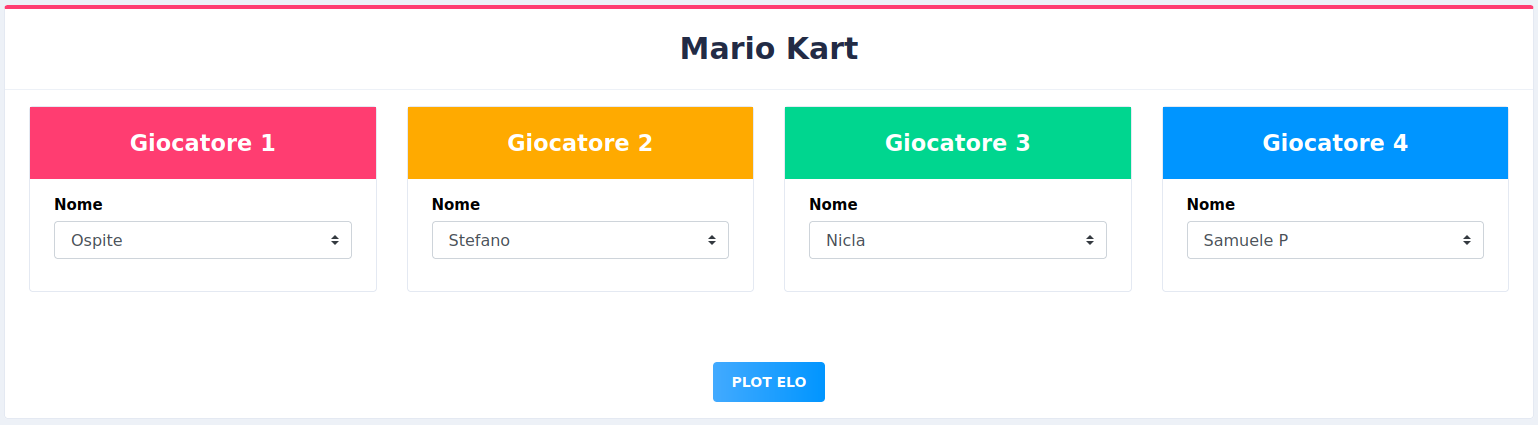
\includegraphics[width=\textwidth]{immagini/insPartita.png} \\
			\caption{\label{fig:inserimento} Form per l'inserimento di una nuova partita}
		\end{figure}
		
		\paragraph{Predizione dei risultati di nuove partite} ~\smallskip 
		
		\noindent Nell'applicativo è presente un algoritmo di \emph{Machine Learning} che, utilizzando i punteggi elo dei giocatori partecipanti, è in grado di predire i risultati della partita.
		Ogni volta che vengono inserite nuove partite, l'algoritmo migliora le proprie predizioni diventando sempre più preciso. 
		
		\begin{figure}[H]
			\centering
			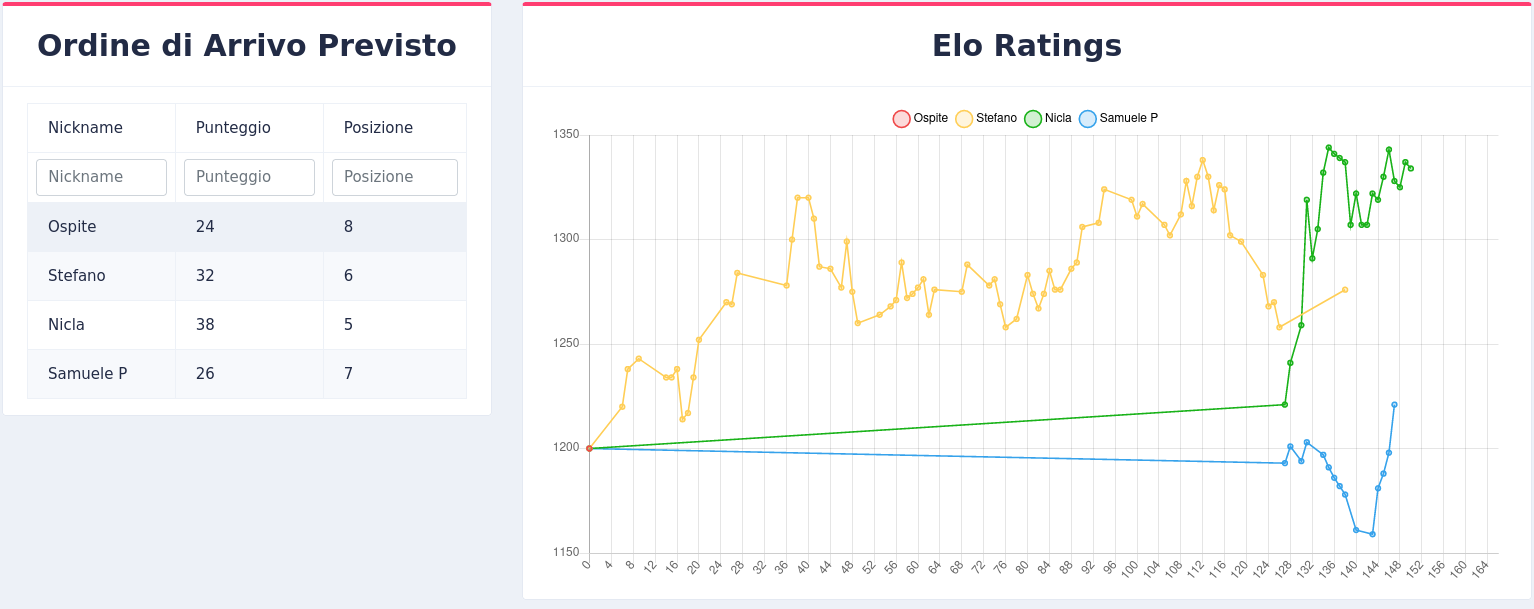
\includegraphics[width=\textwidth]{immagini/predizione.png} \\
			\caption{\label{fig:predizione} Visualizzazione della predizione di una nuova partita}
		\end{figure}
		
		\paragraph{Visualizzazione delle statistiche} ~\smallskip 
		
		\noindent Per ciascun gioco supportato all'interno della web app è presente la pagina \emph{Elo rating}
		che permette di visualizzare i punteggi Elo di tutti i giocatori. Inoltre, sempre all'interno della stessa 
		pagina viene mostrato un grafico con lo storico di tutti i punteggi per i dieci giocatori più frequenti per 
		lo specifico gioco scelto.
		
		\begin{figure}[H]
			\centering
			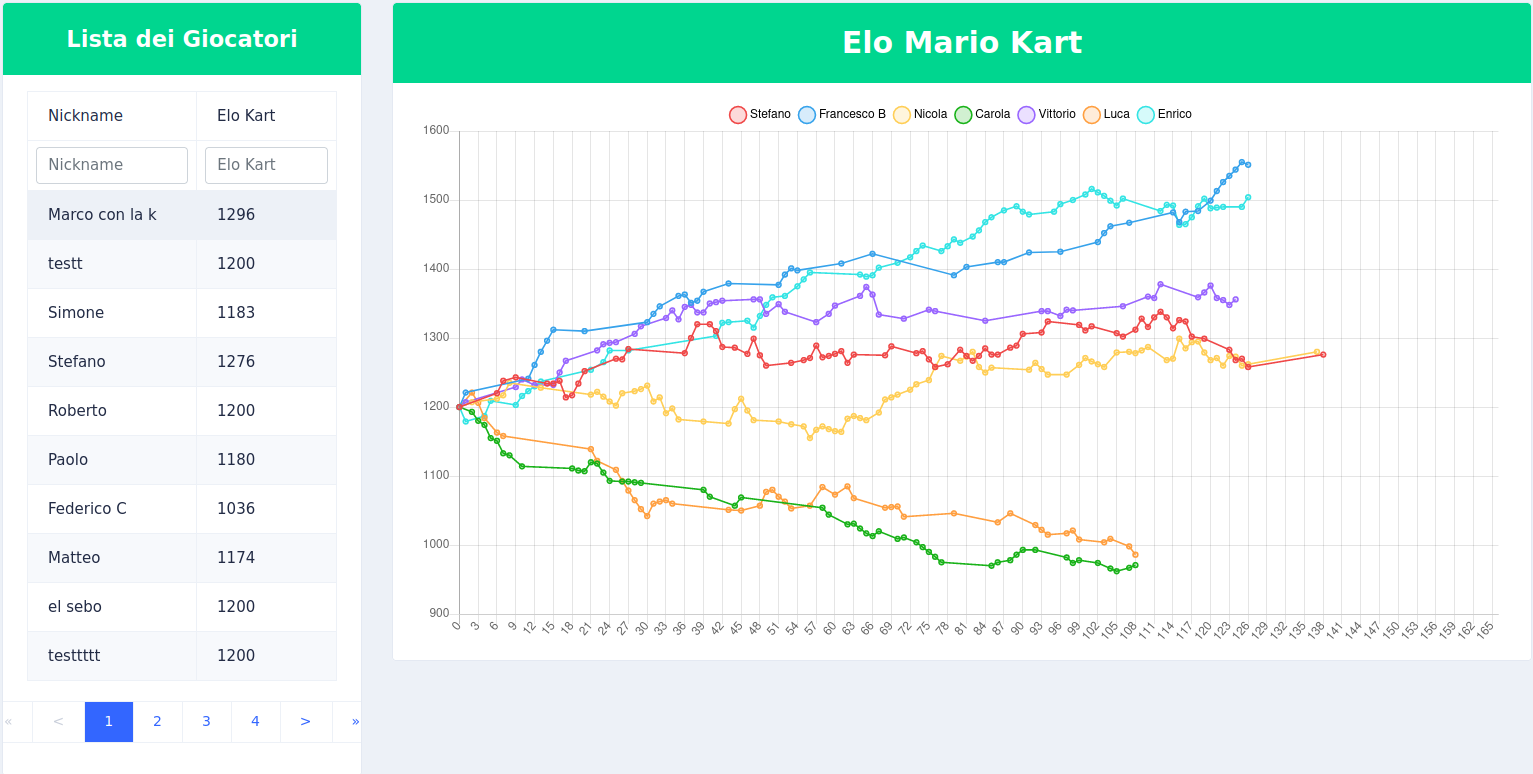
\includegraphics[width=\textwidth]{immagini/elo.png} \\
			\caption{\label{fig:elo} Pagina per la visualizzazione dei punteggi Elo}
		\end{figure}
		
		
	\subsection{Deploy del front-end}
	Per eseguire il \gls{deploy} delle modifiche al front-end è necessario seguire i seguenti passi:
	\begin{enumerate}
		\item Nella cartella del progetto, generare la cartella \emph{dist} eseguendo il comando
		\begin{center}
			\texttt{ng build}
		\end{center}
		\item Utilizzare la console \gls{AWS} per visualizzare il contenuto del bucket in cui è stato eseguito l'hosting del sito;
		\item Sostituire il contenuto del bucket con i file presenti nella cartella \emph{dist} generata;
		\item Utilizzare il servizio \gls{CloudFront} per creare un'\emph{invalidation} e comunicare che i
		contenuti del sito sono cambiati. In questo modo il servizio permetterà di visualizzare le modifiche effettuate.
	\end{enumerate}